\documentclass[a4paper,11pt]{article}

\usepackage[utf8]{inputenc}
\usepackage[T1]{fontenc}
\usepackage[danish,english]{babel}
\usepackage{graphicx}
\usepackage[a4paper,margin=2.7cm]{geometry}
\usepackage[math]{kurier}
\usepackage{amsmath}
\usepackage{amssymb}
\usepackage{amsfonts}
\usepackage{enumerate}
\usepackage{array}
\usepackage{tikz}
\usepackage{booktabs}
\usepackage{float}
\usepackage{lastpage}
\usepackage{listings}
\usepackage{fancyhdr}
\usepackage[ruled,vlined,linesnumbered]{algorithm2e}
\usepackage{longtable}
\usepackage{placeins}
\usepackage{hyperref}

\newcounter{algorithm}
\renewcommand{\thealgorithm}{\arabic{algorithm}}

\usetikzlibrary{arrows,decorations.pathmorphing,backgrounds,positioning,fit,matrix}

\setlength{\parindent}{0pt}
\setlength{\parskip}{2ex} 

\renewcommand{\vec}[1]{\ensuremath {\mathbf #1}}

\newcommand{\courseid}{DM872}
\newcommand{\coursename}{Mathematical Optimization at Work}
\newcommand{\term}{Spring 2025}
\newcommand{\dept}{Department of Mathematics and Computer Science}

\author{Domonkos Kertész}
\newcommand{\assnr}{2}
\makeatletter
\let\runauthor\@author
\let\runtitle\@title
\makeatother

\lstset{language=Python,
  basicstyle=\ttfamily\lst@ifdisplaystyle\footnotesize\fi,
  stringstyle=\ttfamily,
  commentstyle=\ttfamily,
  showstringspaces=false,
  frame=lines, 
  breaklines=true, tabsize=2,
  extendedchars=true,inputencoding=utf8
}

\pagestyle{fancy}
\renewcommand{\sectionmark}[1]{\markright{#1}}
\fancyhf{}
\fancyhead[R]{\runauthor}
\cfoot{Page \thepage\ of \pageref{LastPage}}

\fancypagestyle{plain}{
\lhead{\dept\\
University of Southern Denmark, Odense}
\chead{}
\rhead{\today\\
\runauthor}
\lfoot{}
\rfoot{}
}

\title{\begin{flushleft}
\vspace{-4ex}
\courseid~-- \coursename \\[0.2cm]
{\Large Answers to Obligatory Assignment \assnr, \term \\[3ex]
\hrule}
\end{flushleft}
}

\date{29.05.2025.}

\begin{document}
\maketitle
\setlength{\headheight}{26pt}

\newpage

All files are available on my \href{https://github.com/KihiraLove/SDU-Works/tree/main/Mathematical%20Optimization/ClassWork/Assignment_2}{GitHub}

\section{Determining Solution}

\paragraph{Problem Description}
A delivery company must satisfy orders for 200 retail stores. Each store has a demand that must be served by exactly one truck, and trucks have uniform capacity \(Q=12\,600\) kg. Stores specify \emph{time windows} during which they can receive shipments; some have multiple disjoint intervals. Travel distances are Euclidean based on provided coordinates, and trucks travel at 1000 distance‐units per hour. Service times at each customer are also given in 24h format, and trucks may wait if they arrive early.  

\paragraph{Problem Formulation}
Formulating the VRPTW as a single‐commodity flow MIP with:
\begin{itemize}
  \item Binary variables \(x_{ij}\in\{0,1\}\) indicating whether a vehicle travels from node \(i\) to \(j\).
  \item Continuous variables \(t_i\) for service start times at node \(i\).
  \item Continuous variables \(l_i\) for cumulative load after servicing node \(i\).
  \item Continuous ordering variables \(u_i\) (MTZ) to eliminate subtours.
  \item Binary variables \(y_i\) indicating if customer \(i\) is served (allows skipping with penalty).
\end{itemize}

\paragraph{Objective}
\[
\min 
\sum_{i\neq j} d_{ij}\,x_{ij}
\;+\;P\sum_{i=1}^n (1 - y_i)
\]
where \(d_{ij}\) is Euclidean distance and \(P\) is a large penalty for skipping.

\paragraph{Constraints}
\begin{enumerate}
  \item \textbf{Routing continuity:} \(\sum_j x_{ij}=\sum_j x_{ji}=y_i\) for all customers \(i\).  
  \item \textbf{Depot:} At least one departure and return arc; no self‐loop at depot.
  \item \textbf{Time windows:} \(e_i \le t_i \le \ell_i\) for consolidated interval \([e_i,\ell_i]\).
  \item \textbf{Service propagation:} If \(x_{ij}=1\), then 
    \[
      t_j \ge t_i + s_i + \frac{d_{ij}}{v} - M\,(2 - x_{ij} - y_i - y_j),
    \]
    where \(s_i\) is service time and \(v=1000/60\) units/minute.
  \item \textbf{Capacity:} \(l_0=0\), \(l_i \ge q_i\,y_i\), \(l_i \le Q\), and if \(x_{ij}=1\):
    \[
      l_j \ge l_i + q_j - Q\,(2 - x_{ij} - y_i - y_j).
    \]
  \item \textbf{Subtour elimination (MTZ):} \(1 \le u_i \le n-1\) and 
    \[
      u_i - u_j + (n-1)\,x_{ij} \le n-2 + n\,(2 - y_i - y_j).
    \]
\end{enumerate}

\paragraph{Solution Methodology}
I've adopted the Miller–Tucker–Zemlin formulation for subtour elimination, augmented with big‐M constraints to enforce time‐window and load propagation only when an arc is used and both endpoints are served.

\newpage

\section{Implementing solution}
The implementation is written in Python using Gurobi 12.0.1 as a solver.
\begin{itemize}
  \item \texttt{load\_data()}, \texttt{merge\_data()} and \texttt{compute\_matrices()} parse and preprocess coordinate, demand, service‐time, and raw time‐window files into consolidated DataFrames and distance/travel‐time matrices.  
  \item \texttt{consolidate\_time\_windows()} merges potentially multiple intervals per customer into a single \([e_i,\ell_i]\) by taking the global minimum start and maximum end.  
  \item \texttt{check\_capacity()} asserts no single demand exceeds \(Q=12\,600\).  
  \item \texttt{build\_model()} creates Gurobi variables, objective, and all constraints as outlined above.  
  \item \texttt{solve\_and\_extract()} runs with a 300 s time limit, prints the total penalized distance, reconstructs routes by following variables \(x_{ij}\), and outputs per‐vehicle routes.  
\end{itemize}
This code is fully contained in \texttt{asg2.py}, it is not included in the report itself because I couldn't get TeXworks to render it.

\newpage
 Pseudo code for each function.
 \\
\begin{algorithm}[H]
 \KwData{$\text{time\_str}$: string formatted as “HH:MM”}
 \KwResult{$m$: integer minutes since midnight}
 initialization\;
 split $\text{time\_str}$ on “:” into $h,\,m’$\;
 $h \leftarrow \text{int}(h)$; \quad $m’ \leftarrow \text{int}(m’)$\;
 $m \leftarrow h \times 60 + m’$\;
 \Return $m$\;
 \caption{ \texttt{time\_to\_minutes}}
\end{algorithm}

\begin{algorithm}[H]
 \KwData{Paths: \texttt{coord\_path}, \texttt{demand\_path}, \texttt{service\_path}, \texttt{tw\_path}}
 \KwResult{Tuple of DataFrames $(\mathrm{df\_coordinates},\ \mathrm{df\_demands},\ \mathrm{df\_service\_times},\ \mathrm{df\_time\_windows\_raw})$}
 initialization\;
 \tcp{Define file paths and load each into a DataFrame}
 \ForEach{path in \{\texttt{coord\_path}, \texttt{demand\_path}, \texttt{service\_path}, \texttt{tw\_path}\}}{
   load text file at \texttt{path} into a DataFrame with appropriate column names\;
 }
 apply \texttt{time\_to\_minutes} to the \texttt{start} and \texttt{end} columns of \texttt{df\_time\_windows\_raw}\;
 \Return the four DataFrames\;
 \caption{ \texttt{load\_data}}
\end{algorithm}

\begin{algorithm}[H]
 \KwData{DataFrames \texttt{df\_coordinates}, \texttt{df\_demands}, \texttt{df\_service\_times}}
 \KwResult{Merged DataFrame \texttt{df} sorted by \texttt{id}}
 initialization\;
 $df \leftarrow \texttt{df\_coordinates}$\;
 merge $df$ with \texttt{df\_demands} on \texttt{id}\;
 merge result with \texttt{df\_service\_times} on \texttt{id}\;
 sort $df$ by \texttt{id} ascending\;
 reset row indices of $df$\;
 \Return $df$\;
 \caption{ \texttt{merge\_data}}
\end{algorithm}

\begin{algorithm}[H]
 \KwData{DataFrame \texttt{df\_instances} with columns \texttt{x}, \texttt{y}}
 \KwResult{Matrices $(D, T)$: distances and travel times}
 initialization\;
 extract coordinates array $C \leftarrow \texttt{df\_instances[['x','y']].to\_numpy()}$\;
 \For{$i \leftarrow 0$ \KwTo $n-1$}{
  \For{$j \leftarrow 0$ \KwTo $n-1$}{
    $D[i][j] \leftarrow \text{EuclideanDistance}(C[i], C[j])$\;
  }
 }
 $v \leftarrow 1000/60$\;  \tcp{speed in units/minute}
 \ForAll{$i,j$}{
  $T[i][j] \leftarrow D[i][j] / v$\;
 }
 \Return $(D, T)$\;
 \caption{ \texttt{compute\_matrices}}
\end{algorithm}

\begin{algorithm}[H]
 \KwData{Raw time windows \texttt{df\_time\_windows\_raw}, array of node IDs \texttt{ids}}
 \KwResult{List \texttt{TW} of consolidated $(\text{start},\text{end})$ per node}
 initialization\;
 \ForEach{$i$ in \texttt{ids}}{
  $raw[i] \leftarrow$ empty list\;
 }
 \tcp{Group intervals by node}
 \ForEach{row in \texttt{df\_time\_windows\_raw}}{
  append $(\text{row.start},\text{row.end})$ to $raw[\text{row.id}]$\;
 }
 \ForEach{$i$ in \texttt{ids}}{
  $S \leftarrow \min\{s : (s,e)\in raw[i]\}$\;
  $E \leftarrow \max\{e : (s,e)\in raw[i]\}$\;
  append $(S,E)$ to \texttt{TW}\;
 }
 \Return \texttt{TW}\;
 \caption{ \texttt{consolidate\_time\_windows}}
\end{algorithm}

\begin{algorithm}[H]
 \KwData{DataFrame \texttt{df\_instances} with column \texttt{demand}, capacity $C$}
 \KwResult{Assertion that no single demand exceeds $C$}
 initialization\;
 \If{there exists a demand $d$ in \texttt{df\_instances.demand} such that $d > C$}{
   \textbf{raise AssertionError}("Customer demand exceeds capacity")\;
 }
 \caption{ \texttt{check\_capacity}}
\end{algorithm}

\begin{algorithm}[H]
 \KwData{Parameters: $n$, $D$, $T$, \texttt{df\_instances}, \texttt{TW}, $C$, $M$, $P$}
 \KwResult{Gurobi Model $\mathcal{M}$ and variable dict $\texttt{arc\_used}$}
 initialization\;
 create Gurobi model $\mathcal{M}$ named “VRPTW”\;
 add binary vars $\texttt{arc\_used}[i,j]$ for all $i,j\in[0..n)$\;
 add continuous vars $\texttt{arrival}[i],\,\texttt{load}[i],\,\texttt{mtz}[i]$\;
 add binary vars $\texttt{served}[i]$ for $i\in[1..n)$\;
 set objective: minimize $\sum D[i][j]\cdot \texttt{arc\_used}[i,j] + P\sum(1-\texttt{served}[i])$\;
 \tcp{Routing continuity}
 \For{$i=1$ \KwTo $n-1$}{
  add constraint $\sum_j \texttt{arc\_used}[j,i] = \texttt{served}[i]$\;
  add constraint $\sum_j \texttt{arc\_used}[i,j] = \texttt{served}[i]$\;
 }
 \tcp{Depot constraints}
 add constraint $\sum_{j=1}^{n-1}\texttt{arc\_used}[0,j]\ge1$\;
 add constraint $\sum_{i=1}^{n-1}\texttt{arc\_used}[i,0]\ge1$\;
 set $\texttt{arc\_used}[0,0].ub\leftarrow0$\;
 \tcp{Time windows}
 \For{$i=0$ \KwTo $n-1$}{
  $(s,e)\leftarrow \texttt{TW}[i]$\;
  add constraint $\texttt{arrival}[i]\le e$\;
 }
 add constraint $0 \le \texttt{arrival}[0]\le M$\;
 \tcp{Capacity}
 add constraint $\texttt{load}[0]=0$\;
 \For{$i=1$ \KwTo $n-1$}{
  add constraint $\texttt{load}[i]\ge \texttt{df\_instances.demand}[i]\cdot \texttt{served}[i]$\;
  add constraint $\texttt{load}[i]\le C$\;
 }
 \tcp{Propagation along arcs}
 \For{$i=1$ \KwTo $n-1$}{
  \For{$j=1$ \KwTo $n-1$, $j\neq i$}{
    add time constraint with big-$M$ condition\;
    add load constraint with big-$M$ condition\;
  }
 }
 \tcp{MTZ subtour elimination}
 \For{$i=1$ \KwTo $n-1$}{
  add constraints $1\le \texttt{mtz}[i]\le n-1$\;
  \For{$j=1$ \KwTo $n-1$}{
    add MTZ constraint with arc and served variables\;
  }
 }
 \Return $(\mathcal{M}, \texttt{arc\_used})$\;
 \caption{ \texttt{build\_model}}
\end{algorithm}

\begin{algorithm}[H]
 \KwData{Gurobi Model $\mathcal{M}$, $\texttt{arc\_used}$, distance matrix $D$}
 \KwResult{Printed routes or infeasibility report}
 initialization\;
 set solver time limit to 300 seconds\;
 $\mathcal{M}.\text{optimize()}$\;
 \eIf{$\mathcal{M}.\text{status}\in\{\text{OPTIMAL},\text{TIME\_LIMIT}\}$}{
  print total distance\;
  identify all routes by tracing $\texttt{arc\_used}[0,j]$ from depot\;
  \ForEach{route found}{
   compute route length using $D$\;
   print vehicle route and length\;
  }
 }{
  \eIf{$\mathcal{M}.\text{status}=\text{INFEASIBLE}$}{
   print “Model infeasible”; compute and write IIS file\;
  }{
   print “No solution found.”\;
  }
 }
 \caption{ \texttt{solve\_and\_extract}}
\end{algorithm}

\paragraph{Computational Results}
Running on a 4‐thread Intel i7‐6500U, the solver explored 1 635 nodes in 300 s, producing:
\begin{itemize}
  \item \textbf{Total distance (with penalties):} 142\,479.83  
  \item \textbf{Number of vehicles:} 51  
  \item \textbf{Optimality gap:} 85.98\%  
\end{itemize}

\newpage
Vehicle routes (distance in units):

\begin{longtable}{lrr}
\caption{Vehicle distances and routes}\label{tab:routes}\\
\hline
Vehicle & Distance & Route sequence \\ 
\hline
\endfirsthead
\multicolumn{3}{c}%
  {{\bfseries \tablename\ \thetable{} -- continued from previous page}}\\
\hline
Vehicle & Distance & Route sequence \\ 
\hline
\endhead
\hline \multicolumn{3}{r}{{Continued on next page}} \\ 
\endfoot
\hline
\endlastfoot
1 & 612.96 &[0,4,76,41,0]\\
2 & 2\,649.06 &[0,6,1,9,23,0]\\
3 & 6\,359.65 &[0,8,15,28,71,86,0]\\
4 & 1\,346.87 &[0,13,52,64,62,0]\\
5 & 607.83 &[0,17,54,55,0]\\
6 & 2\,085.12 &[0,21,34,5,2,0]\\
7 & 480.13 &[0,22,38,27,10,0]\\
8 & 898.94 &[0,24,11,0]\\
9 & 1\,691.11 &[0,25,20,3,14,16,43,0]\\
10 & 604.76 &[0,31,48,33,0]\\
11 & 1\,801.11 &[0,44,35,37,56,0]\\
12 & 1\,129.63 &[0,51,42,57,0]\\
13 & 2\,575.77 &[0,53,40,45,0]\\
14 & 6\,502.11 &[0,59,26,29,18,0]\\
15 & 2\,467.99 &[0,61,46,36,39,47,0]\\
16 & 3\,890.60 &[0,63,30,32,0]\\
17 & 2\,744.21 &[0,68,65,88,112,0]\\
18 & 1\,687.12 &[0,78,60,50,0]\\
19 & 3\,276.73 &[0,79,70,87,129,0]\\
20 & 2\,272.79 &[0,81,69,73,100,0]\\
21 & 5\,763.38 &[0,83,80,82,170,0]\\
22 & 1\,040.41 &[0,89,84,77,58,0]\\
23 & 1\,718.63 &[0,90,111,94,85,0]\\
24 & 1\,317.74 &[0,95,103,91,66,7,0]\\
25 & 2\,960.83 &[0,97,96,147,138,0]\\
26 & 1\,164.03 &[0,99,105,92,74,0]\\
27 & 1\,879.24 &[0,102,107,93,0]\\
28 & 2\,624.73 &[0,104,110,116,0]\\
29 & 4\,515.66 &[0,109,67,19,106,0]\\
30 & 1\,509.56 &[0,113,121,120,98,0]\\
31 & 2\,497.87 &[0,114,124,141,145,146,125,0]\\
32 & 3\,555.21 &[0,122,123,117,135,0]\\
33 & 2\,981.01 &[0,128,134,126,0]\\
34 & 2\,879.64 &[0,137,130,133,139,0]\\
35 & 1\,543.70 &[0,144,154,148,0]\\
36 & 1\,594.31 &[0,149,140,142,72,0]\\
37 & 2\,598.91 &[0,155,156,152,0]\\
38 & 3\,258.30 &[0,157,132,101,115,162,0]\\
39 & 2\,855.07 &[0,158,160,150,108,0]\\
40 & 5\,460.43 &[0,159,136,119,49,12,0]\\
41 & 1\,914.80 &[0,164,175,153,75,0]\\
42 & 4\,922.77 &[0,167,151,118,131,0]\\
43 & 5\,083.99 &[0,169,163,143,127,182,0]\\
44 & 4\,485.79 &[0,176,168,161,179,0]\\
45 & 4\,208.37 &[0,177,174,165,0]\\
46 & 3\,225.93 &[0,178,192,181,171,0]\\
47 & 4\,343.46 &[0,185,173,187,0]\\
48 & 3\,643.99 &[0,186,193,184,172,166,0]\\
49 & 3\,982.62 &[0,188,183,180,0]\\
50 & 3\,627.95 &[0,197,190,195,196,198,0]\\
51 & 3\,636.99 &[0,199,189,191,194,0]\\
\end{longtable}

\newpage
\section{Visualization of Results}
Figure~\ref{fig:all_routes} shows the combined solution. Figures for each route can be found bellow.

\begin{figure}[H]
  \centering
  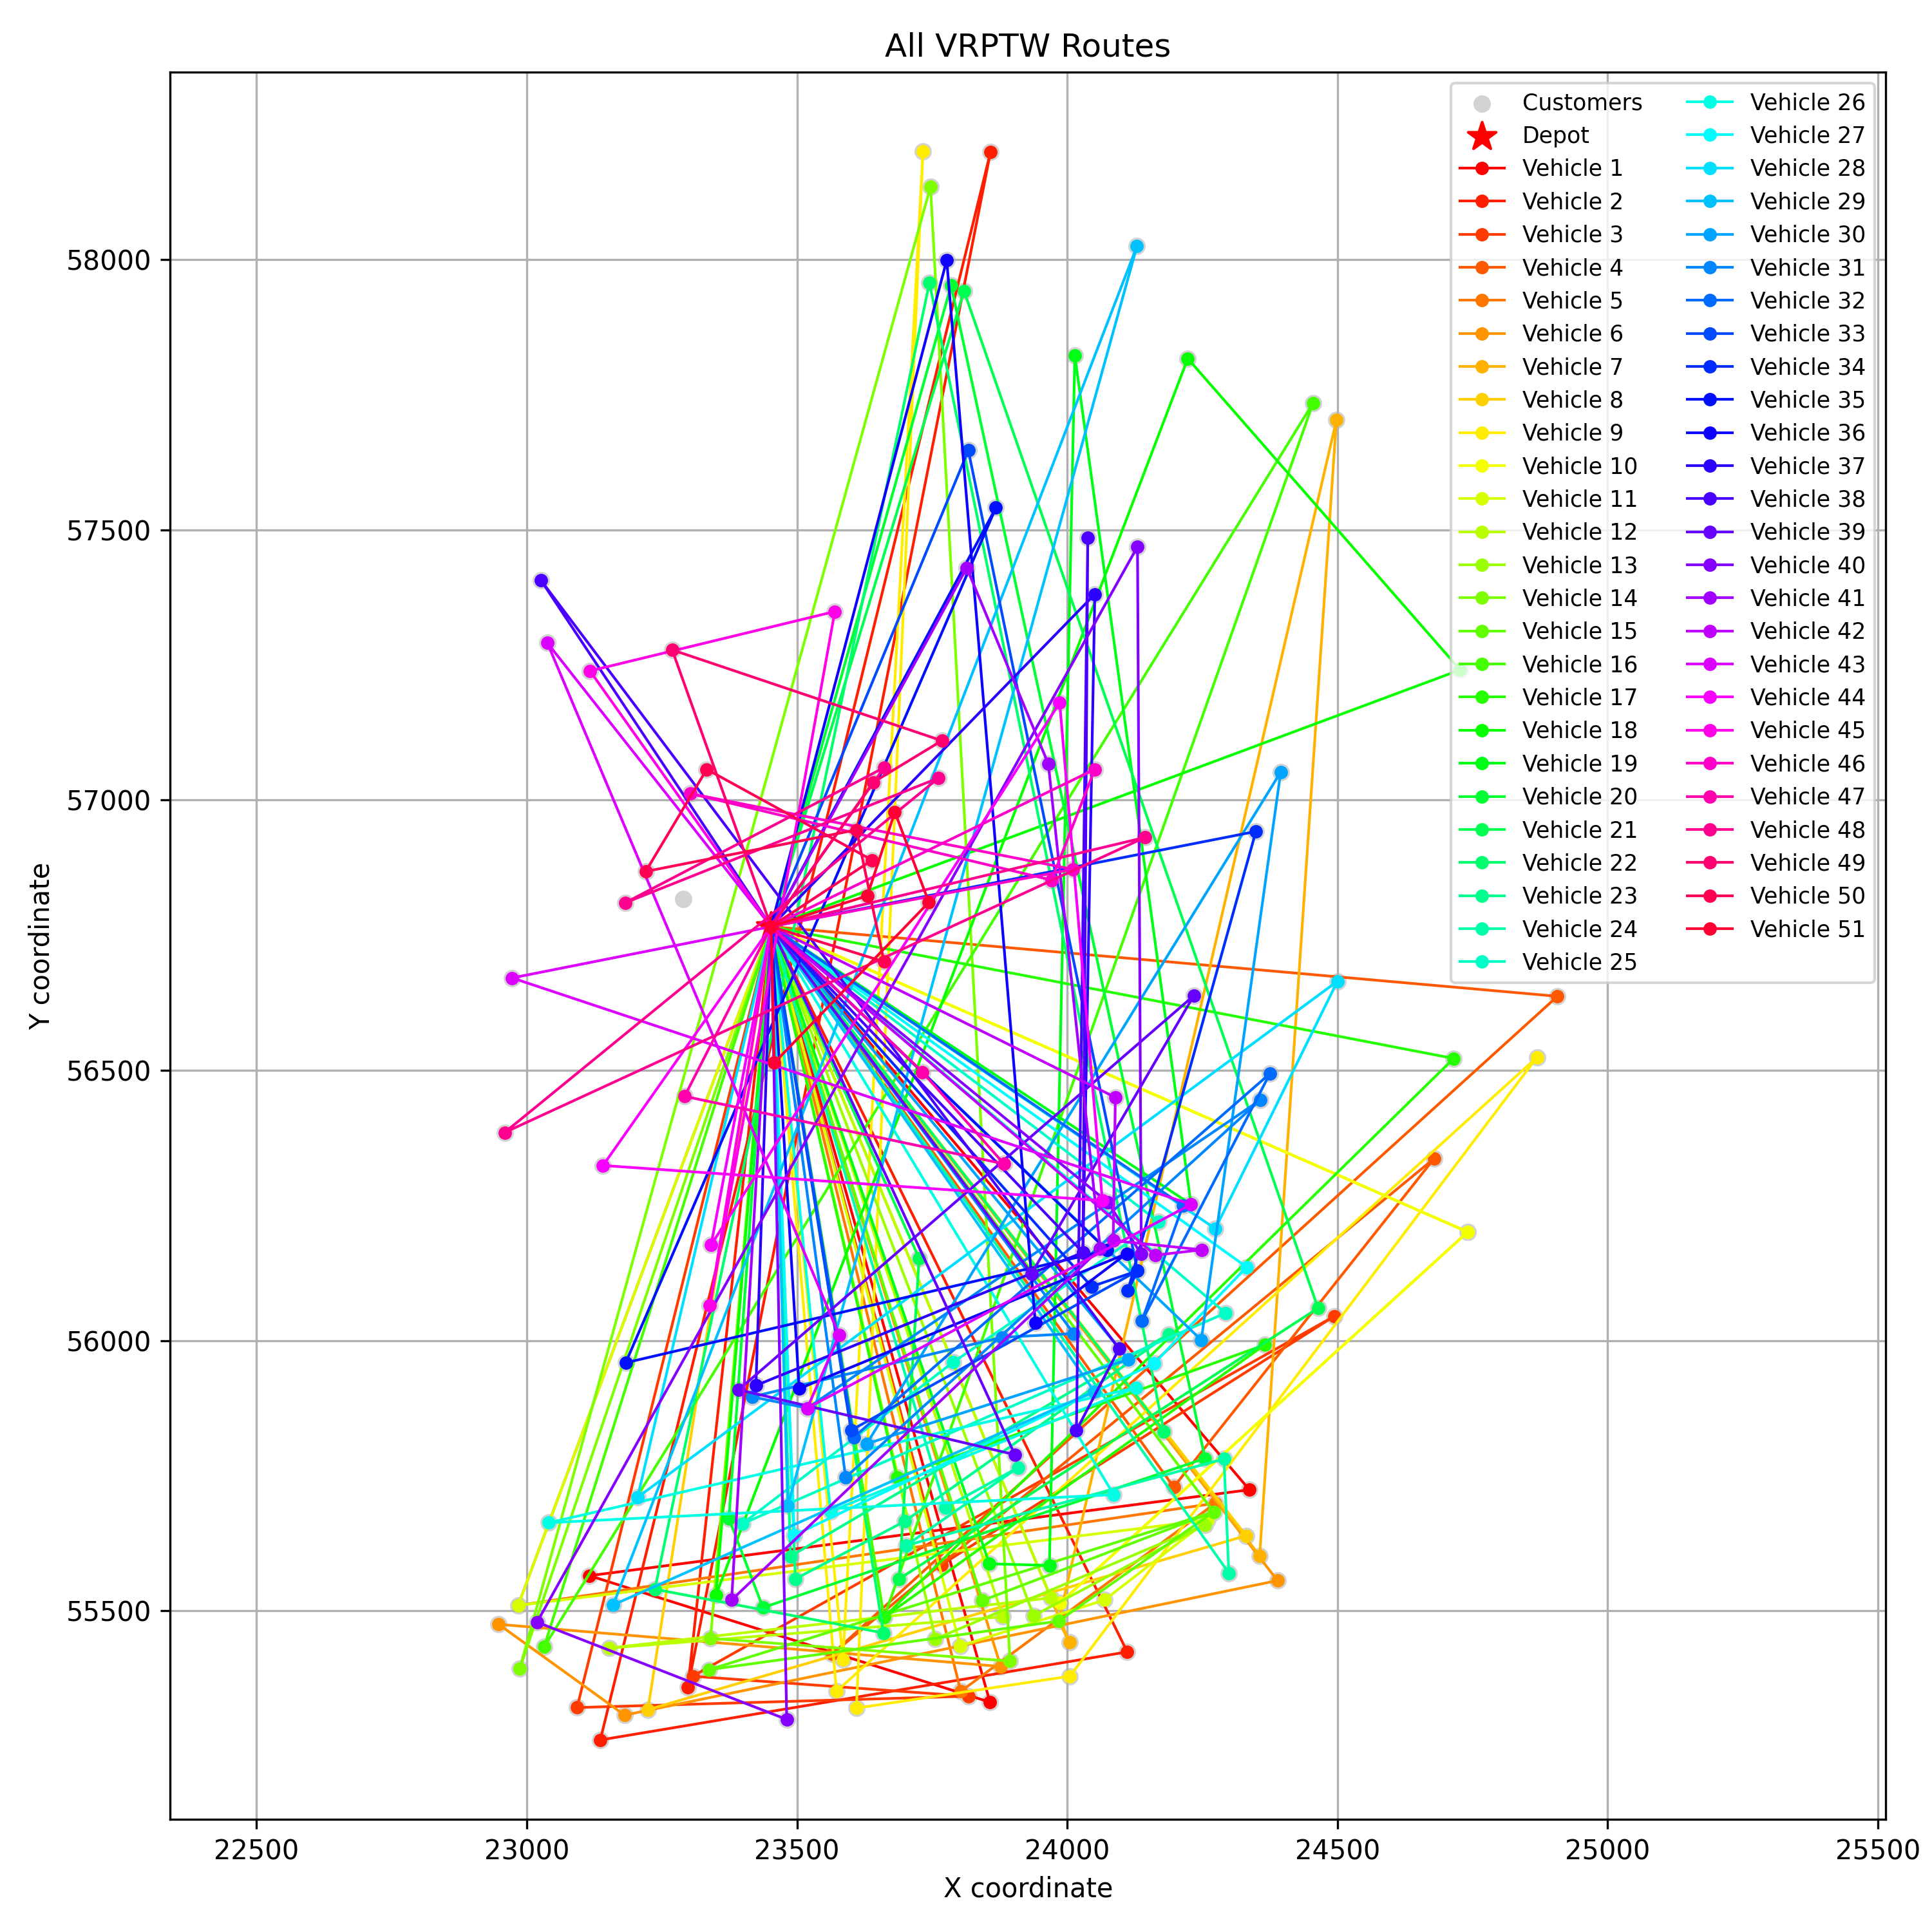
\includegraphics[width=0.9\linewidth]{plots/all_routes.png}
  \caption{Combined VRPTW solution routes}
  \label{fig:all_routes}
\end{figure}

\newpage

\begin{figure}[H]
  \centering
  \setlength{\parindent}{0pt}%
  \foreach \i in {1,...,15}{%
    \begin{minipage}{0.30\linewidth}
      \centering
      \includegraphics[width=\linewidth]{plots/route_\i.png}
    \end{minipage}%
    \ifnum\i=3\par\fi
    \ifnum\i=6\par\fi
    \ifnum\i=9\par\fi
    \ifnum\i=12\par\fi
    \ifnum\i=15\par\fi
  }
  \caption{Individual routes for each vehicle (1--15)}
  \label{fig:single_routes}
\end{figure}

\newpage

\begin{figure}[H]
  \centering
  \setlength{\parindent}{0pt}%
  \foreach \i in {16,...,30}{%
    \begin{minipage}{0.30\linewidth}
      \centering
      \includegraphics[width=\linewidth]{plots/route_\i.png}
    \end{minipage}%
    \ifnum\i=18\par\fi
    \ifnum\i=21\par\fi
    \ifnum\i=24\par\fi
    \ifnum\i=27\par\fi
    \ifnum\i=30\par\fi
  }
  \caption{Individual routes for each vehicle (16--30)}
  \label{fig:single_routes}
\end{figure}

\newpage

\begin{figure}[H]
  \centering
  \setlength{\parindent}{0pt}%
  \foreach \i in {31,...,45}{%
    \begin{minipage}{0.30\linewidth}
      \centering
      \includegraphics[width=\linewidth]{plots/route_\i.png}
    \end{minipage}% 
    \ifnum\i=33\par\fi
    \ifnum\i=36\par\fi
    \ifnum\i=39\par\fi
    \ifnum\i=42\par\fi
    \ifnum\i=45\par\fi
  }
  \caption{Individual routes for each vehicle (31--45)}
  \label{fig:single_routes}
\end{figure}

\newpage

\begin{figure}[H]
  \centering
  \setlength{\parindent}{0pt}%
  \foreach \i in {46,...,51}{%
    \begin{minipage}{0.30\linewidth}
      \centering
      \includegraphics[width=\linewidth]{plots/route_\i.png}
    \end{minipage}% 
    \ifnum\i=48\par\fi
    \ifnum\i=51\par\fi
  }
  \caption{Individual routes for each vehicle (46--51)}
  \label{fig:single_routes}
\end{figure}

\end{document}
          



